TODO: Add that all data is captured after one minute of warm-up, and learning rate is fixed to 0.005, dicussed in Limitations (see Section \ref{sec:limitations}), experiment duration, calibration duration

This chapter presents the empirical evaluation of the proposed adaptive consensus architecture. The primary goal is to evaluate whether risk-controlled mode prediction can capitalize on specific operating conditions where fast-path execution offers latency advantages without exceeding target failure rates.

The adaptive system is evaluated against two static protocol baselines. The first baseline represents a Regular Paxos implementation using a trimmed-down version of the OmniPaxos \cite{Ng-OmniPaxos-2023} codebase, where all followers consistently forward proposals to the central leader via the regular path. The second baseline is a static Fast Paxos implementation in which all followers unconditionally attempt fast-path broadcasts for every proposal. 

After presenting the detailed experimental setup (see Section \ref{sec:experimental_setup}). The evaluation examines the system across four key performance and correctness dimensions. First, we assess whether the score function is a useful heuristic under dynamic request rates in Section \ref{sec:score_function_validity}. Second, Section \ref{sec:risk_guarantee_validity} verifies whether the Rolling Risk Control layer strictly bounds long-term empirical fast-path failure rates to the user-specified risk level. Third, Section \ref{sec:latency_study} analyzes end-to-end request latencies across European and US cluster topologies to identify the specific operational scenarios where adaptive mode switching achieves performance gains. Finally, Section \ref{sec:overhead_analysis} concludes the chapter by quantifying the possible overhead that can be introduced by the adaptive mechanism.


\section{Experimental Setup}
\label{sec:experimental_setup}
The evaluation prototype is implemented in the Rust programming language, building directly upon a trimmed-down fork of the original OmniPaxos \cite{Ng-OmniPaxos-2023} codebase. To cleanly isolate the protocol variables associated with decentralized mode switching, several production-level features of OmniPaxos were omitted. The log is managed entirely via an in-memory storage layer, which enforces a fail-stop failure model where nodes do not recover from persistent disk state. Because the evaluation assumes a stable leader, a fully safe log synchronization phase at the conclusion of the prepare phase was omitted. Additionally, request batching is disabled, ensuring that performance evaluation isolates fine-grained end-to-end latency rather than aggregate throughput.

Building upon this baseline, the consensus layer incorporates the required protocol interoperability and modification rules outlined previously. This includes adding the AcceptStatus field in both Accept and Accepted messages, implementing the followers' logic to broadcast proposals directly to peers via the fast path, and executing the tracking and deterministic collision-detection logic defined in Algorithm \ref{alg:quorum_eval_collision_resolution} and Algorithm \ref{alg:leader_proposal} on the leader side. Follower-side update semantics are enforced to maintain safety: followers reject standard FastAccept and LeaderAccept messages if the target log index is already occupied, but permit SlowAccept commands from the leader to override existing entries during collision resolution.

When we operate in adaptive mode, the system implements dedicated tracking mechanisms for network features and success labels. To estimate the fast-quorum latency, the \gls{BLE} layer extends its standard heartbeat messages with a timestamp. Upon receiving a reply, the round-trip time is divided by two to compute individual one-way network latencies. Concurrently, the sequence Paxos layer tracks a running count of incoming Accept requests received within a sliding one-second window to estimate the proposal rate of other cluster nodes. Next to the shadow proposals, ground-truth labels are gathered by analyzing the final AcceptStatus of a node's own completed proposals once they are decided, where a resolved FastAccept signifies a fast-path success.

These features and labels are processed by the prediction layer implemented as an isolated module. The module evaluates the model and executes the decision framework outlined in Algorithm \ref{alg:conformal_mode_prediction}. In the offline calibration phase, the system executes a binary root-finding algorithm over a pre-collected batch dataset of feature-label pairs to establish the initial baseline threshold. During runtime operations, an online calibration routine continuously updates the threshold as described previously.

\subsection{State Machine Application}
\begin{figure}[t!]
    \centering
    \begin{tikzpicture}
    \node[anchor=south west, inner sep=0] (map) at (0,0) {
\includegraphics[width=\textwidth]{figures/BlankMap-Europe.pdf}};
    
    \tikzset{
        server info/.style={
            align=center,
            font=\sffamily\scriptsize
        },
        edge label/.style={
            fill=white,
            text=gray!90!black,
            font=\sffamily\scriptsize\bfseries,
            inner sep=2pt,
            rounded corners=2pt,
            draw=gray!20,
            thin
        }
    }

    \node[label={[server info]right:\textbf{Madrid} (ID: 2)\\europe-southwest1-b}] (madrid) at (1.5, 1.0) {
        
\includegraphics[width=1.2cm]{figures/cluster_node.pdf}
    };
    
    \node[label={[server info]left:\textbf{London} (ID: 3)\\europe-west2-b}] (london) at (3.5, 8.0) {
        
\includegraphics[width=1.2cm]{figures/cluster_node.pdf}
    };
    
    \node[label={[server info]below:\textbf{Frankfurt} (ID: 5)\\europe-west3-b}] (frankfurt) at (8.0, 7.0) {
        
\includegraphics[width=1.2cm]{figures/cluster_node.pdf}
    };
    
    \node[label={[server info]below:\textbf{Warsaw} (ID: 4)\\europe-central2-b}] (warsaw) at (11.75, 8.0) {
        
\includegraphics[width=1.2cm]{figures/cluster_node.pdf}
    };
    
    \node[label={[server info]left:\textbf{Stockholm} (ID: 1)\\europe-north2-b}] (stockholm) at (11.5, 12.0) {
        
\includegraphics[width=1.2cm]{figures/cluster_node.pdf}
    };

    \begin{scope}[every path/.style={{Triangle}-{Triangle}, draw=blue!50!gray, thick}]
        
        \draw (madrid) -- (london) node[midway, edge label] {12ms};
        \draw (frankfurt) -- (warsaw) node[midway, edge label] {10ms};
        \draw (warsaw) -- (stockholm) node[midway, edge label] {13ms};
        
        \draw (madrid) to[bend left=12] node[midway, edge label] {24ms} (stockholm);
        \draw (madrid) to[bend right=8] node[midway, edge label] {20ms} (warsaw);
        \draw (madrid) to[bend left=12] node[midway, edge label] {12ms} (frankfurt);
        
        \draw (london) to[bend left=10] node[midway, edge label] {6ms} (frankfurt);
        \draw (london) to[bend left=10] node[midway, edge label] {17ms} (stockholm);
        \draw (london) to[bend left=10] node[midway, edge label] {13ms} (warsaw);
        
        \draw (frankfurt) to[bend right=10] node[midway, edge label] {14ms} (stockholm);
    \end{scope}
    
    \node[orange, rotate=20, xshift=0.2cm] at (frankfurt.north west) {\large\faCrown};
\end{tikzpicture}
    \caption{European cluster setup, including one-way latencies.}
    \label{fig:europe-cluster-setup}
\end{figure}

For the experiments, we used a linearizable, in-memory key-value store as the application-level replicated state machine. State transitions and queries are driven by three basic operations: inserting a key-value pair, deleting a key, or retrieving a value based on a key. To guarantee strict linearizability and prevent stale data, both read and write operations are appended to the consensus log. As the consensus engine commits these entries, the server executes the commands sequentially once they are decided.

Client requests are encapsulated into a standardized command structure that includes a unique command identifier and a coordinator node identifier. Upon receiving a request, the coordinator node appends this command to the consensus log. After the log entry is committed and executed sequentially by the state machine, the node matching the recorded coordinator identifier handles routing the final execution outcome back to the originating client.

\subsection{Node Setup}
\label{sect:node_setup}
\begin{figure}[t]
    \centering
    \begin{tikzpicture}
    \node[anchor=south west, inner sep=0] (map) at (0,0) {
\includegraphics[width=\textwidth]{figures/BlankMap-US.pdf}};
    
    \tikzset{
        server info/.style={
            align=center,
            font=\sffamily\scriptsize
        },
        edge label/.style={
            fill=white,
            text=gray!90!black,
            font=\sffamily\scriptsize\bfseries,
            inner sep=2pt,
            rounded corners=2pt,
            draw=gray!20,
            thin
        }
    }

    \node[label={[server info]left:\textbf{Oregon} (ID: 1)\\us-west1-b}] (oregon) at (3.0, 6.5) {
        
\includegraphics[width=1.2cm]{figures/cluster_node.pdf}
    };
    
    \node[label={[server info]below:\textbf{Los Angeles} (ID: 3)\\us-west2-b}] (los-angeles) at (1.25, 3.0) {
        
\includegraphics[width=1.2cm]{figures/cluster_node.pdf}
    };
    
    \node[label={[server info]above:\textbf{Iowa} (ID: 3)\\us-central1-b}] (iowa) at (10.0, 6.0) {
        
\includegraphics[width=1.2cm]{figures/cluster_node.pdf}
    };
    
    \node[label={[server info]below:\textbf{Columbus} (ID: 4)\\us-east5-b}] (columbus) at (11.75, 3.75) {
        
\includegraphics[width=1.2cm]{figures/cluster_node.pdf}
    };
    
    \node[label={[server info]below:\textbf{Las Vegas} (ID: 5)\\us-west4-b}] (las-vegas) at (4.0, 4.0) {
        
\includegraphics[width=1.2cm]{figures/cluster_node.pdf}
    };

    \begin{scope}[every path/.style={{Triangle}-{Triangle}, draw=blue!50!gray, thick}]
        
        \draw (oregon) -- (los-angeles) node[midway, edge label] {12ms};
        \draw (columbus) -- (iowa) node[midway, edge label] {11ms};
        \draw (los-angeles) -- (las-vegas) node[midway, edge label] {4ms};
        \draw (oregon) -- (columbus) node[midway, edge label] {31ms};
        
        \draw (las-vegas) to[bend left=10] node[midway, edge label] {30ms} (columbus);
        \draw (oregon) to[bend left=20] node[midway, edge label] {19ms} (iowa);
        \draw (oregon) to[bend left=12] node[midway, edge label] {13ms} (las-vegas);
        \draw (los-angeles) to[bend right=14] node[midway, edge label] {23ms} (iowa);
        \draw (los-angeles) to[bend right=25] node[midway, edge label] {32ms} (columbus);
        \draw (las-vegas) to[bend left=20] node[midway, edge label] {14ms} (iowa);
    \end{scope}
    
    \node[orange, rotate=20, xshift=0.2cm] at (las-vegas.north west) {\large\faCrown};
\end{tikzpicture}
    \caption{US cluster setup, including one-way latencies.}
    \label{fig:us-cluster-setup}
\end{figure}

To evaluate the system under realistic yet stable network conditions, the prototype is deployed on \gls{GCP} homogeneous \texttt{e2-standard-4} instances running Debian 13, as detailed in Table \ref{tab:hardware-software-setup}. This instance class provides four virtual CPUs, guaranteeing at least one dedicated core per system component to prevent thread-scheduling bottlenecks. The network is configured with Google Virtual NICs and the Premium routing tier, ensuring that observed latency variances stem from geographic distance and workload contention rather than artificial cloud provider jitter. 

Architecturally, the system on each node is decoupled into three distinct Docker containers (\texttt{client}, \texttt{server}, and \texttt{daemon}) using host networking to bypass virtualization overhead. The network daemon persists connections between nodes across different experiment runs, eliminating connection-establishment variance that would otherwise skew baseline latencies. Inter-process communication between the server and daemon is handled locally via Unix Domain Sockets.

\begin{table}[t]
\centering
\renewcommand{\arraystretch}{1.2}
\begin{tabular}{ll}
\toprule
\textbf{Component} & \textbf{Configuration} \\
\midrule
Cloud Provider & Google Cloud Platform \\
Machine Type & \texttt{e2-standard-4} (4 vCPUs, 16\,GB RAM) \\
Operating System & Debian 13 \\
Boot Disk Size & 10\,GB \\
Network Interface Type & Google Virtual NIC \\
Network Routing Tier & Premium\\
Provisioning Model & Standard \\
Container Environment & Docker (\texttt{--network host}) \\
\bottomrule
\end{tabular}
\caption{Hardware and software configuration specifications for the experimental cluster instances deployed on GCP.}
\label{tab:hardware-software-setup}
\end{table}

The evaluation is conducted across two distinct 5-node clusters, located in Europe (Figure \ref{fig:europe-cluster-setup}) and the US (Figure \ref{fig:us-cluster-setup}), to provide diverse latency profiles. Given a cluster size of $n=5$, a majority quorum requires three nodes for the regular and slow paths, while the fast path requires a strict fast quorum of four nodes. Because this thesis represents an exploratory study of the protocol's performance viability, the evaluation strictly assumes a zero-failure environment. This isolates the adaptive mechanism under ideal operating conditions, leaving availability trade-offs for future work. To explore realistic routing conditions, the stable leader is deterministically assigned to the most geographically central node in each cluster: Frankfurt in Europe and Las Vegas in the US.


\begin{table}[t]
\centering
\renewcommand{\arraystretch}{1.2}
\begin{tabular}{lccc}
\toprule
\textbf{Node} & \textbf{Regular Path} & \textbf{Fast Path} & \textbf{Slow Path} \\
\midrule
Stockholm  & 48ms & \textbf{\textit{40ms}} & 60ms \\
Madrid  & 46ms & \textbf{\textit{44ms}} & 64ms \\
London  & 38ms & \textbf{\textit{35ms}} & 55ms \\
Warsaw  & 40ms & \textbf{\textit{37ms}} & 57ms \\
Frankfurt  & \textbf{\textit{20ms}}  & 26ms & 46ms \\ 
\bottomrule
\end{tabular}
\caption{Estimated end-to-end latencies in the European cluster setup using regular, fast, or slow execution paths for an entry appended by a co-located client.}
\label{tab:cluster-latencies-europe}
\end{table}


\begin{table}[t]
\centering
\renewcommand{\arraystretch}{1.2}
\begin{tabular}{lccc}
\toprule
\textbf{Node} & \textbf{Regular Path} & \textbf{Fast Path} & \textbf{Slow Path} \\
\midrule
Oregon  & \textbf{\textit{52ms}} & 53ms & 79ms \\
Los Angeles  & \textbf{\textit{21ms}} & 48ms & 74ms \\
Iowa  & 68ms & \textbf{\textit{53ms}} & 79ms \\
Columbus  & 86ms & \textbf{\textit{66ms}} & 92ms \\
Las Vegas  & \textbf{\textit{26ms}} & 42ms & 68ms \\ 
\bottomrule
\end{tabular}
\caption{Estimated end-to-end latencies in the US cluster setup using regular, fast, or slow execution paths for an entry appended by a co-located client.}
\label{tab:cluster-latencies-us}
\end{table}

Tables \ref{tab:cluster-latencies-europe} and \ref{tab:cluster-latencies-us} present the estimated baseline latencies from the perspective of a co-located client. This end-to-end measurement encapsulates the initial request, quorum gathering (fast or regular), potential collision resolution, the leader's decide phase, local execution, and the final reply to the client. Co-locating the client simulates the architectural pattern of routing requests to the nearest edge replica while satisfying practical resource constraints.

The European topology exhibits a relatively distributed latency profile, where followers uniformly gain a slight advantage on a successful fast path because broadcasting to a localized fast quorum is faster than forwarding. Conversely, the US topology has a more polarized profile. While distant nodes benefit significantly from the fast path, nodes physically close to the leader, such as Oregon and Los Angeles, incur a latency penalty when attempting to gather four distributed votes compared to simply forwarding their request. Since these nodes have zero mathematical incentive to switch operating modes, their local modes are locked to Regular Paxos in the adaptive experiments.

\subsection{Workload Pattern}
\begin{figure*}[t!]
    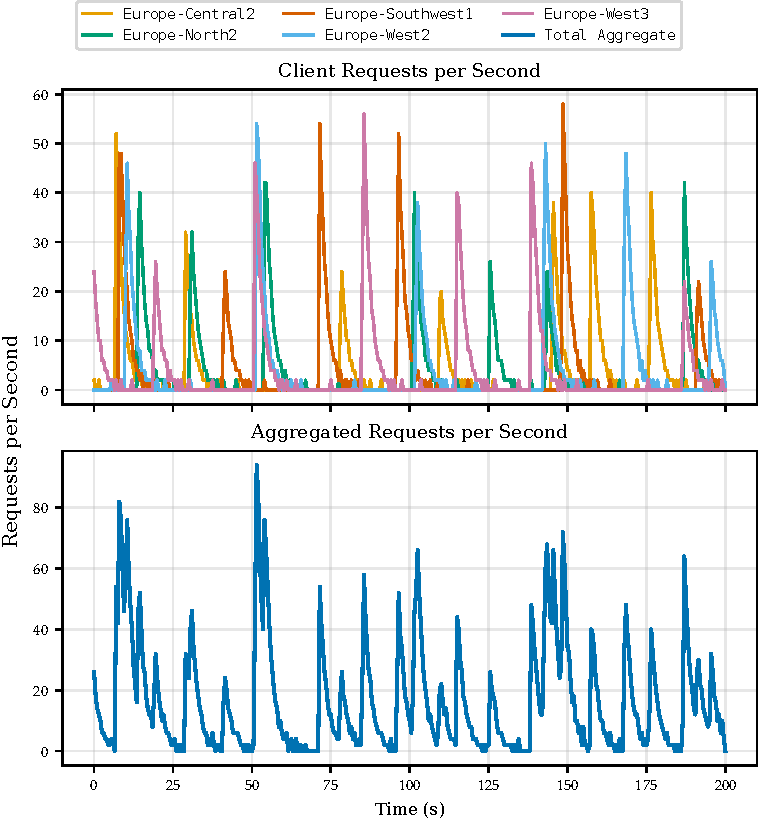
\includegraphics[width=\linewidth]{figures/client_load_localevents.pdf}
    \caption{Sample of the client workload pattern used for experimentation.} 
    \label{fig:workload-pattern}
\end{figure*}

Because the evaluation assesses the viability of an adaptive consensus protocol, the workload must deliberately trigger conditions where the optimal strategy fluctuates between Fast Paxos and Regular Paxos. Under sustained, heavy traffic, standard consensus protocols like OmniPaxos~\cite{Ng-OmniPaxos-2023} or Raft~\cite{Ongaro-Raft-2014} are strictly superior due to high collision rates on the fast path. Consequently, stress-testing maximum throughput is out of scope. Instead, the evaluation employs a highly bursty, low-contention workload to represent ideal conditions for the adaptive system, ensuring periods where the fast path is highly viable are interspersed with periods of high collision risk.

Traffic generation is therefore driven by local events at the clients. To create windows of opportunity for Fast Paxos, the baseline traffic between events is set to zero \gls{RPS}. When a local event triggers at a node, the client injects a rapid burst of 50 peak \gls{RPS}. This simulates a sudden influx of client activity that normalizes along an exponential decay curve with a rate of 0.5. Burst timing is unpredictable: intervals between events are sampled from a normal distribution with a 30-second mean and a 15-second standard deviation. A jitter factor of 0.5 applies randomized variance to the peak height of each burst to further simulate organic traffic.

Each geographic server is driven by a single, independent client process sending requests. This setup does not impact collision rates, as collisions inherently occur across the network between different servers rather than locally. Because each of the nodes generates localized bursts independently, the aggregate system load dynamically fluctuates. Figure \ref{fig:workload-pattern} depicts a sample of this workload pattern, showing both the request trace for individual servers and the overall aggregate load.


\section{Score Function Validity}
\label{sec:score_function_validity}

\section{Risk Guarantee Validity}
\label{sec:risk_guarantee_validity}

\section{Latency Study}
\label{sec:latency_study}

\begin{figure*}[t!]
    \centering
    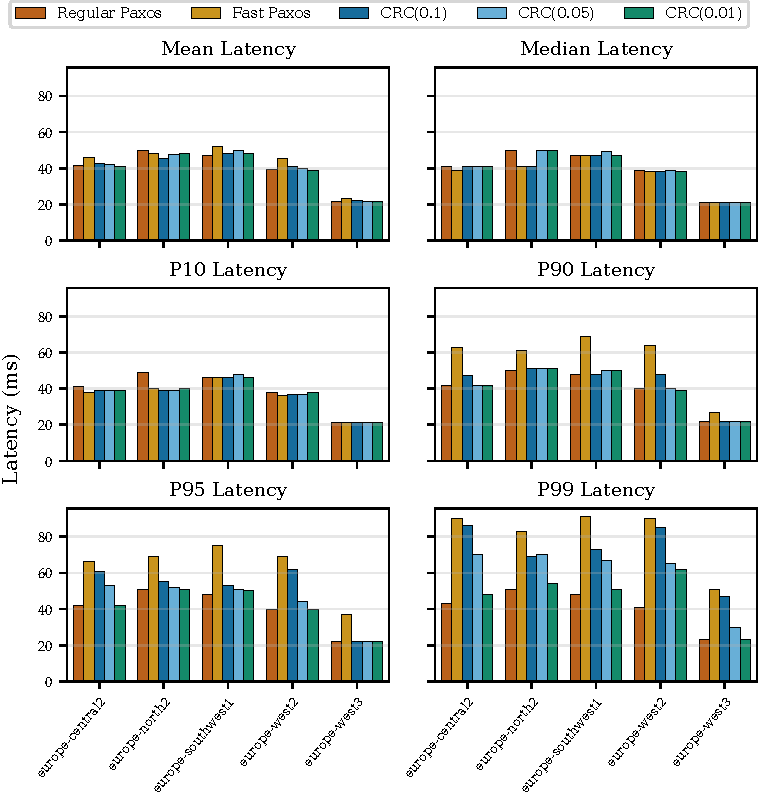
\includegraphics[width=\linewidth]{figures/latency_comparison_europe.pdf}
    \caption{End-to-end latency comparison for the European cluster setup between Regular Paxos, Fast Paxos, and Conformal Consensus with various risk levels.} 
    \label{fig:latency_comparison_europe}
\end{figure*}

We analyze the end-to-end request latencies of Conformal Consensus under different risk levels compared to static Regular Paxos and Fast Paxos baselines. Figures \ref{fig:latency_comparison_europe} and \ref{fig:latency_comparison_us} display the mean, median, and tail latencies (P10, P90, P95, P99) for both regions under the bursty workload pattern described in Section \ref{sec:experimental_setup}.

In the European cluster experiment, Regular Paxos maintains a flat latency profile across all percentiles (P10--P99), demonstrating strong resilience to workload contention. In contrast, static Fast Paxos achieves lower P10 latency for followers but suffers substantial latency inflation at higher percentiles (P90, P95, and P99), producing the widest overall latency spread. This can also be seen at the leader node (\texttt{europe-west3}). Because high-percentile penalties heavily impact the average, static Fast Paxos reduces mean latency only when the geographic fast-path advantage is substantial, as seen at the Stockholm node (\texttt{europe-north2}). Where fast-path benefits are marginal, its mean latency regresses relative to Regular Paxos.

Conformal Consensus dampens these extreme tail latencies. At a conservative risk level ($\alpha = 0.01$), for instance, latency inflation is restricted strictly to the P99 tail and remains unobservable at P90 and P95. Simultaneously, the adaptive mechanism preserves the low P10 latency of Fast Paxos, successfully capturing and increasing mean latency improvements on nodes with large fast-path advantages. However, where fast-path gains are minimal, residual slow-path fallbacks at high percentiles still cause a slight regression in mean latency compared to pure Regular Paxos.

Finally, the target risk level $\alpha$ establishes a direct trade-off between stability and latency reduction. Lowering $\alpha$ systematically increases tail dampening and tightens the overall latency spread toward Regular Paxos, though this added stability proportionally diminishes potential mean latency gains.

\begin{figure*}[t!]
    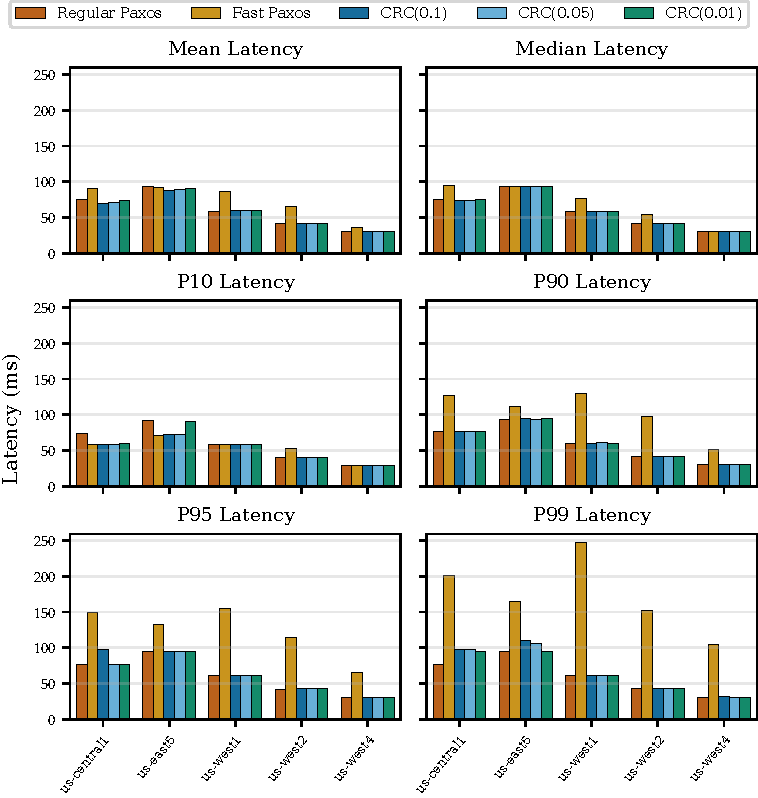
\includegraphics[width=\linewidth]{figures/latency_comparison_us.pdf}
    \caption{End-to-end latency comparison for the (simulated) US cluster setup between Regular Paxos, Fast Paxos, and Conformal Consensus with various risk levels.} 
    \label{fig:latency_comparison_us}
\end{figure*}

To mitigate the unpredictable cloud network variance observed in the US cluster setupc, all nodes were deployed within a single geographic zone (\texttt{us-west4-c}) for the latency experiment, with the regional latency profile injected application-side. Under these conditions, the Regular and Fast Paxos baselines exhibit the same general performance trends observed in the European cluster.

As discussed in Section \ref{sect:node_setup}, the Conformal Consensus configuration continuously routes \texttt{us-west1}, \texttt{us-west2}, and the leader (\texttt{us-west4}) through the regular path. The latencies for these nodes perfectly mirror the Regular Paxos baseline across all percentiles through the added stability. For the actively adapting nodes, higher theoretical fast-path gains result in a noticeable reduction in mean latency, making Conformal Consensus outperform both static baselines in this specific setup.


\section{Overhead Analysis}
\label{sec:overhead_analysis}
Conformal Consensus can introduce overhead in two primary areas: per-request mode evaluation during follower append attempts and threshold computation during batch calibration.

\begin{figure*}[t]
    \centering
    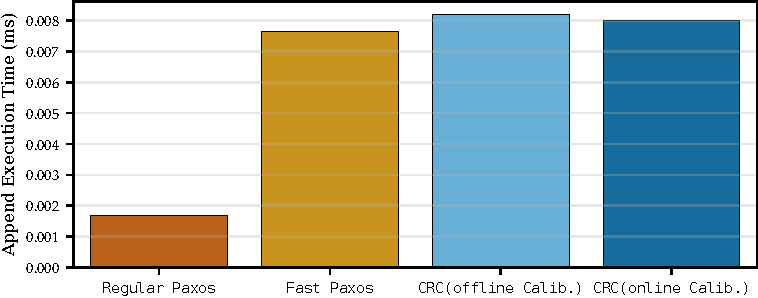
\includegraphics[width=\linewidth]{figures/append_performance.pdf}
    \caption{Average execution times of an append attempt by followers across operating modes.} 
    \label{fig:append_performance}
\end{figure*}

Figure~\ref{fig:append_performance} shows the average local execution time per append attempt on a follower across operating modes. Regular Paxos requires under $0.002\,\text{ms}$ because the follower only forwards incoming requests to the leader. Fast Paxos increases this due to proposal broadcasting among peers. Adding \gls{CRC}, which includes evaluating the heuristic score, generating the prediction set, and processing potential shadow proposals during offline calibration, incurs less than $0.01\,\text{ms}$ of combined compute overhead per request. Given that end-to-end network latencies in both cluster topologies are on the order of tens of milliseconds (Section~\ref{sec:experimental_setup}), this local compute overhead is negligible and has no practical impact on request latency.

\begin{figure*}[t]
    \centering
    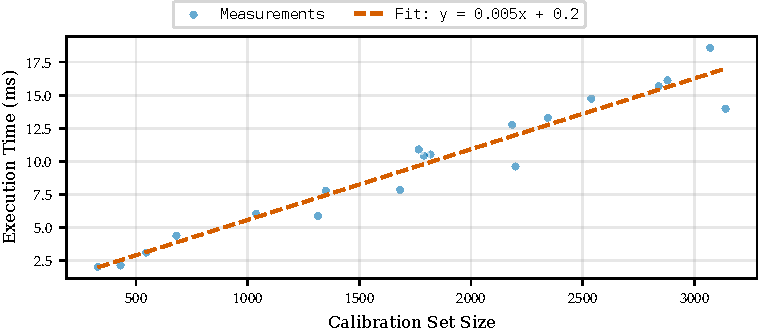
\includegraphics[width=\linewidth]{figures/calibration_overhead.pdf}
    \caption{Threshold computation time during batch calibration relative to calibration set size.} 
    \label{fig:calibration_overhead}
\end{figure*}

The second potential source of overhead is batch calibration, which runs a binary root-finding algorithm to establish an initial threshold $\widehat{\lambda}$. As shown in Figure~\ref{fig:calibration_overhead}, execution time scales linearly with dataset size. For a dataset of 3,000 samples (collected over 15 minutes under described workload patterns), the algorithm computes the threshold in approximately $15\,\text{ms}$. Batch calibration is entirely optional and serves primarily to establish a reliable baseline threshold prior to running online calibration. Because data collection can occur during regular operations, the root-finding routine can execute asynchronously, and the computational load is this low, batch calibration introduces no runtime disruption to the main consensus path.